  Now, we will show \ref{eqn:gallai-proof-2}. Let \(X\) be the minimum edge 
  cover of \(G\). Then, we have \(|X|=\beta'(G)=l\). Let \(F = G[X]\) or a 
  subgraph induced by \(X\). Notice that \(F\) has no
  trail of length 3. Otherwise, there must be a middle edge \(e\) but \(X
  \setminus \{e\}\) would still be an edge cover of \(G\), creating a
  contradiction. Hence, \(F\) contains no cycle and no paths of length 3 or
  grater. This implies that every component of \(F\) is a star. 

  Notice that each component with \(n_i\) vertices has \(n_i - 1\) edges. So,
  if \(F\) has \(c\) components, then it has \(n-c\) edges and all of these must
  be in the edge cover. Hence, we have that
  \[
  \begin{aligned}
    l \geq n-c \iff c \geq n-l
  \end{aligned}
  \]
  To find \(\alpha'(G)\), we can pick one edge from each component of \(F\).
  Then, it follows that 
  \[ \alpha'(G) = c \geq n-l \]
  This implies that 
  \[ \alpha'(G) + \beta'(G) \geq (n-l) + l = n \] 
\end{proof}

\begin{theorem}
  For every graph \(G\) of order \(n\) containing no isolated vertices, we have
  \[ \alpha(G) + \beta(G) = n \]
\end{theorem}

\begin{proof}
  The proof is similar to Gallai's Theorem and will be omitted.
\end{proof}

\begin{nexample}
  Prove that if \(G\) is a graph of order \(n\) with maximum degree \(\Delta\)
  and has no isolated vertices, then 
  \[ \beta(G) \geq \frac{n}{\Delta + 1} \]

  \begin{proof}
    Let \(G\) be a graph of order \(n\) and suppose that \(G\) has \(k\)
    components. We make the following observations:
    \begin{enumerate}
      \item \(|E(G)| \leq \beta(G) \cdot \Delta\). This is because
        \(\beta(G)\) gives the number of vertices needed to cover every edge,
        and each vertex has at most \(\Delta\) edges incident to it.
      \item \(n-k \leq |E(G)|\). Notice that \(n-k\) is the minimum number of
        edges required for a graph with \(k\) components to have no isolated
        vertices.
      \item \(k \leq \beta(G)\). Otherwise, there would be isolated vertices
        with violates our assumption.
    \end{enumerate}
    Combining all of these together, we have that
    \[ n-\beta(G) \leq n-k \leq |E(G)| \leq \beta(G) \cdot \Delta \]
    Finally, we have that 
    \[
    \begin{aligned}
      n - \beta(G) &\leq \beta(G) \cdot \Delta \\ 
      n &\leq \beta(G) (\Delta + 1) \\ 
      \frac{n}{\Delta + 1} &\leq \beta(G)
    \end{aligned}
    \]
    which is the inequality we wanted to show.
  \end{proof}
\end{nexample}

\begin{remark}
  The bound in the example is weak when \(G\) has many edges. 
\end{remark}

\chapter{Connectivity}

\section{Bridges and Cut-vertices}

\begin{definition}[Bridge]
  An edge \(e = (u, v)\) or \(uv\) of a connected graph \(G\) is
  called a \textit{bridge} of \(G\) if \(G - e\) is disconnected.
\end{definition}

\begin{figure}[ht]
\begin{nexample}
  Here is a disconnected graph with 4 bridges.

  \centering
  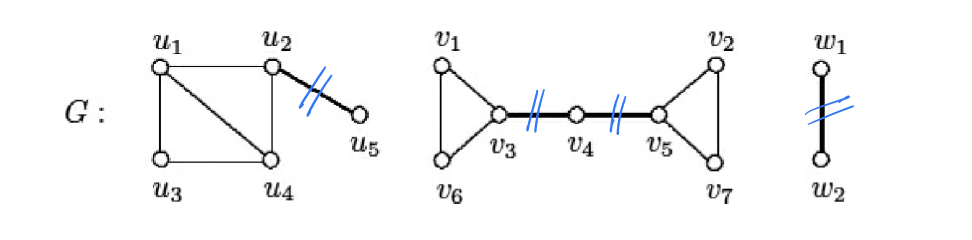
\includegraphics[width=0.69\textwidth]{figures/l09/bridge-examples}
\end{nexample}
\end{figure}

\begin{theorem}
  An edge \(e\) of a graph \(G\) is a bridge if and only if \(e\)
  lies on no cycle of \(G\).
\end{theorem}

\begin{proof}
  If \(e\) lies on a cycle, then \(e\) cannot be a bridge since
  we can always find an \textit{alternate} path between any two
  vertices that are part of \(G\) so \(G-e\) would still be
  connected.

  Similarly, if \(e=xy\) is not a bridge and there is another
  path \(P\) from \(x\) to \(y\), then \(P \cup {xy}\) forms a
  cycle that contains \(e\).
\end{proof}

\begin{definition}[Cut-vertex]
  A vertex \(v\) in a connected graph \(G\) is a
  \textit{cut-vertex} of \(G\) if \(G-v\) is disconnected.
  This can be thought of as the vertex version of a bridge.
\end{definition}

\begin{figure}[ht]
\begin{nexample}
  Here is an example of a graph \(G\) and \(G-v\).

  \centering
  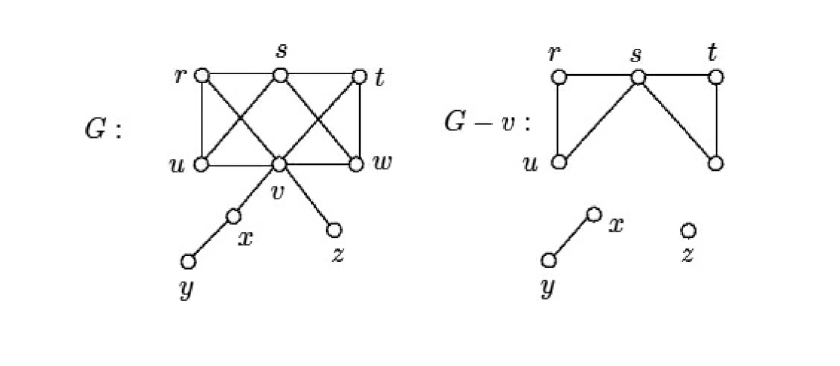
\includegraphics[width=0.69\textwidth]{figures/l09/cut-vertex-example}
\end{nexample}
\end{figure}

\begin{remark}
  For a tree \(T\), every non-leaf vertex \(v\) is a cut-vertex.
\end{remark}

\begin{theorem}
  Let \(v\) be a vertex incident with a bridge in a connected
  graph \(G\). Then, \(v\) is a cut-vertex of \(G\) if and only
  if \(\deg v \geq 2\).
\end{theorem}

\begin{proof}
  If \(\deg v = 1\), then \(v\) is an end point and cannot be a
  cut-vertex. Otherwise, suppose that the bridge that \(v\) is
  incident to is \(e=uv\). Then, \(G-v\) would also not have
  \(e\) which makes the graph disconnected. Thus, \(v\) is a
  cut-vertex.
\end{proof}

\begin{corollary}
  Let \(G\) be a connected graph of order 3 or more. If \(G\)
  conatains a bridge, then \(G\) contains a cut-vertex.
\end{corollary}

\begin{proof}
  Let \(e = xy\) be a bridge. Then, either \(\deg x \geq 2\) or
  \(\deg y \geq 2\). So, either \(x\) or \(y\) must be a
  cut-vertex.
\end{proof}

\begin{theorem}
  Let \(v\) be a cut-vertex in a connected graph \(G\) and let
  \(u, w\) be vertices in distinct components of \(G-v\). Then,
  \(v\) lies on every \(u-w\) path in \(G\).
\end{theorem}

\begin{proof}
  Assume to the contrary that there is a \(u-v\) path that does
  not go through \(v\). Then, \(v\) would not be a cut-vertex
  since \(G-v\) would not be disconnected.
\end{proof}

\begin{corollary}
  A vertex \(v\) of a connected graph \(G\) is a cut-vertex of
  \(G\) if and only if there exists \(u, w\) distinct from \(v\)
  such that \(v\) lies on every \(u-w\) path of \(G\).
\end{corollary}

\section{Vertex-cuts and Edge-cuts}

\begin{definition}[Vertex-cut]
  A \textit{vertex-cut} in a graph \(G\) is a set \(U \subseteq
  V(G)\) such that \(G \setminus U\) is disconnected.
  Additionally, a vertex-cut of minimum cardinality in \(G\) is
  called a \textit{minimum vertex-cut}.
\end{definition}

\begin{definition}[Vertex-connectivity]
  The \textit{vertex-connectivity} (or simply the
  \textit{connectivity}), denoted by \(\kappa(G)\) is the
  cardinality of a minimum vertex-cut of \(G\). Furthermore, a
  graph is said to be \(k\)-connected if \(\kappa(G) \geq k\).
\end{definition}

\begin{remark}
  \(\kappa(K_n)\) is defined to be \(n-1\).
\end{remark}

\begin{figure}[ht]
\begin{nexample}
  Let us identify the \(\kappa(G_i)\) for each \(i=1, 2, 3\).

  \begin{center}
    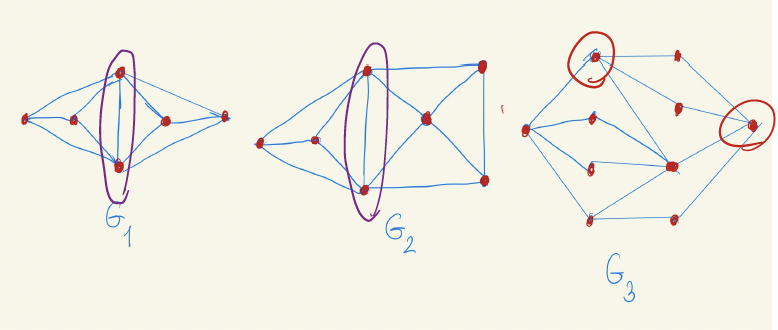
\includegraphics[width=0.69\textwidth]{figures/l09/vertex-connectivity-example}
  \end{center}

  As seen in the diagrams, we can see that
  \[
    \begin{aligned}
      \kappa(G_1) &= 2 \\ 
      \kappa(G_2) &= 2 \\
      \kappa(G_3) &= 2 \\
    \end{aligned}
  \]
  and \(U\) are circled.
\end{nexample}
\end{figure}

\begin{nexample}
  Is there a fixed integer \(M\) such that every graph of minimum
  degree at least \(M\) is 1-connected?

  First, notice that a 1-connected graph means that we need to
  remove at least 1 vertex to disconnect the graph. While it is
  impossible such \(M\) that works for every graph, we can find a
  disconnected graph where \(\delta(G) = M\). Namely, consider a
  disconnected graph where the two components are \(K_{M+1}\)
  graphs.
\end{nexample}
